\documentclass[../notes.tex]{subfiles}

\pagestyle{main}
\renewcommand{\chaptermark}[1]{\markboth{\chaptername\ \thechapter\ (#1)}{}}
\setcounter{part}{2}

\begin{document}




\part{Pinter}
\setcounter{chapter}{2}
\chapter{The Definition of Groups}
\subsection*{Exercises}
\begin{enumerate}[label={\textbf{\Alph*.}}]
    \setcounter{enumi}{3}
    \item \textbf{A Checkerboard Game}
    \begin{center}
        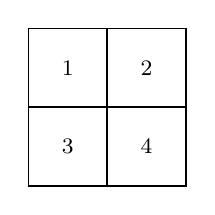
\begin{tikzpicture}[
            every node/.style={draw,semithick,minimum width=1cm,minimum height=1cm}
        ]
            \footnotesize
            \node at (0,1) {1};
            \node at (1,1) {2};
            \node at (0,0) {3};
            \node at (1,0) {4};
        \end{tikzpicture}
    \end{center}
    Our checkerboard has only 4 squares, numbered 1, 2, 3, and 4. There is a single checker on the board, and it has four possible moves:
    \begin{itemize}[itemsep=0pt]
        \item[$V$:] Move vertically; that is, move from 1 to 3, or from 3 to 1, or form 2 to 4, or from 4 to 2.
        \item[$H$:] Move horizontally; that is, move from 1 to 2 or vice versa, or from 3 to 4 or vice versa.
        \item[$D$:] Move diagonally; that is, move from 2 to 3 or vice versa, or from 1 to 4 or vice versa.
        \item[$I$:] Stay put.
    \end{itemize}
    We may consider an operation on the set of these four moves, which consists of performing moves successively. For example, if we move horizontally and then vertically, we end up with the same result as if we had moved diagonally:
    \begin{equation*}
        H*V = D
    \end{equation*}
    If we perform two horizontal moves in succession, we end up where we started: $H*H=I$. And so on. If $G=\{V,H,D,I\}$, and $*$ is the operation we have just described, write the table of $G$. Granting associativity, explain why $\langle G,*\rangle$ is a group.
\end{enumerate}



\chapter{Elementary Properties of Groups}
\begin{itemize}
    \stepcounter{proposition}
    \item \marginnote{7/19:}Let $G$ be a group, and let $a,b\in G$.
    \begin{theorem}
        If $ab=e$, then $a=b^{-1}$ and $b=a^{-1}$.
    \end{theorem}
\end{itemize}



\setcounter{chapter}{8}
\chapter{Isomorphism}
\begin{itemize}
    \item \marginnote{7/20:}\textbf{Isomorphism} (between groups $G_1,G_2$): A bijective function $f:G_1\to G_2$ with the property that for any $a,b\in G_1$, $f(ab)=f(a)f(b)$. \emph{Denoted by} $\bm{G_1\cong G_2}$.
\end{itemize}

\subsection*{Exercises}
\begin{enumerate}[label={\textbf{\Alph*.}}]
    \setenumerate[2]{label={\textbf{\arabic*}}}
    \item \textbf{Isomorphism Is an Equivalence Relation among Groups}
    \begin{enumerate}
        \item Let $G$ be any group. If $\varepsilon:G\to G$ is the identity function, $\varepsilon(x)=x$, show that $\varepsilon$ is an isomorphism.
        \begin{proof}
            To prove that $\varepsilon$ is an isomorphism, it will suffice to show that $\varepsilon$ is a bijection and that $\varepsilon(ab)=\varepsilon(a)\varepsilon(b)$ for all $a,b\in G$. Let $a,b\in G$ be arbitrary. By the definition of $\varepsilon$, $\varepsilon(a)=\varepsilon(b)$ implies $a=b$. Thus, $\varepsilon$ is injective. Additionally, we have that $\varepsilon(b)=b$, so $\varepsilon$ is surjective. Therefore, it is bijective. Lastly,
            \begin{equation*}
                \varepsilon(ab) = ab = \varepsilon(a)\varepsilon(b)
            \end{equation*}
            as desired.
        \end{proof}
        \item Let $G_1,G_2$ be groups, and $f:G_1\to G_2$ be an isomorphism. Show that $f^{-1}:G_2\to G_1$ is an isomorphism.
        \begin{proof}
            Since $f$ is a bijection, $f^{-1}$ exists and is a bijection. Additionally, let $c,d\in G_2$ be arbitrary. Then $f^{-1}(c)=a$ and $f^{-1}(d)=b$ for some $a,b\in G_1$. Thus, since $f(ab)=f(a)f(b)=cd$, we have that $f^{-1}(cd)=f^{-1}(f(ab))=ab=f^{-1}(c)f^{-1}(d)$, as desired.
        \end{proof}
        \item Let $G_1,G_2,G_3$ be groups, and let $f:G_1\to G_2$ and $g:G_2\to G_3$ be isomorphisms. Prove that $g\circ f:G_1\to G_3$ is an isomorphism.
        \begin{proof}
            Since $f,g$ are bijections, $g\circ f$ is a bijection. Now let $a,b\in G_1$ be arbitrary. Thus, $f(ab)=f(a)f(b)$, where $f(a),f(b)\in G_2$. It follows that $g(f(a)f(b))=g(f(a))g(f(b))$. Therefore,
            \begin{equation*}
                (g\circ f)(ab) = g(f(ab))
                = g(f(a)f(b))
                = g(f(a))g(f(b))
                = (g\circ f)(a)(g\circ f)(b)
            \end{equation*}
            as desired.
        \end{proof}
    \end{enumerate}
    \item \textbf{Elements Which Correspond under an Isomorphism}
    \begin{enumerate}
        \item If $e_1$ denotes the neutral element of $G_1$ and $e_2$ denotes the neutral element of $G_2$, prove that $f(e_1)=e_2$.
        \begin{proof}
            For all $x\in G_1$, $e_1x=x=xe_1$. Thus, by the definition of an isomorphism, $f(e_1)f(x)=f(e_1x)=f(x)$ and $f(x)f(e_1)=f(xe_1)=f(x)$. It follows by their definition that $f(e_1)$ is a neutral element of $G_2$. Therefore, since neutral elements are unique, $f(e_1)=e_2$, as desired.
        \end{proof}
        \item Prove that for each element $a\in G_1$, $f(a^{-1})=[f(a)]^{-1}$.
        \begin{proof}
            Let $a\in G_1$ be arbitrary. Then $e_2=f(e_1)=f(aa^{-1})=f(a)f(a^{-1})$. It follows by Theorem 4.2 that $f(a^{-1})=[f(a)]^{-1}$, as desired.
        \end{proof}
        \item If $G_1$ is a cyclic group with generator $a$, prove that $G_2$ is also a cyclic group, with generator $f(a)$.
        \begin{proof}
            Suppose $G_1$ is a cyclic group of order $n$ with generator $a$. We wish to show that $G_2$ is a cyclic group of order $n$ with generator $f(a)$. By the definition of an isomorphism,
            \begin{equation*}
                f(a^t) = f(\underbrace{aa\cdots a}_{t\text{ times}})
                = \underbrace{f(a)f(a)\cdots f(a)}_{t\text{ times}}
                = f(a)^t
            \end{equation*}
            for all $t\in\Z$. As a special case, $e_2=f(e_1)=f(a^n)=f(a)^n$, so $G_2$ is of order \emph{at most} $n$. Now suppose for the sake of contradiction that there exists a positive integer $0<t<n$ such that $f(a)^t=e_2$. Then $f(a^t)=e_2$, i.e., $a^t=e_2$. But this means that $G_1$ is of order $t$, a contradiction.
        \end{proof}
    \end{enumerate}
    \item \textbf{Isomorphism of Some Finite Groups}
    \begin{enumerate}
        \item $G$ is the checkerboard game group of Chapter 3, Exercise D. $H$ is the group of the complex numbers $\{i,-i,1,-1\}$ under multiplication.
        \begin{proof}
            Suppose for the sake of contradiction that an isomorphism $f:G\to H$ exists. Since $-i^1=-i$, $-i^2=-1$, $-i^3=i$, and $-i^4=1$, $H=\langle -i\rangle$. Thus, by Exercise 9.B.3, $G$ is a cyclic group with generator $f^{-1}(-i)$. However, no element $x\in G$ suffices as a generator ($I^1=I$, $V^2=I$, $H^2=I$, and $D^2=I$), a contradiction.
        \end{proof}
    \end{enumerate}
\end{enumerate}



\setcounter{chapter}{12}
\chapter{Counting Cosets}
\begin{itemize}
    \item \marginnote{7/22:}\textbf{Left coset} (of $H$ in $G$): The set of all products $ah$, where $H$ is a subgroup of $G$, $a\in G$ is fixed, and $h$ ranges over $H$. \emph{Denoted by} $\bm{aH}$.
    \item \textbf{Right coset} (of $H$ in $G$): The set of all products $ha$, where $H$ is a subgroup of $G$, $a\in G$ is fixed, and $h$ ranges over $H$. \emph{Denoted by} $\bm{Ha}$.
    \item In this book, we choose to focus on right cosets.
    \item If $a\in Hb$, then $Ha=Hb$.
    \begin{proof}
        Let $x\in Ha$ be arbitrary. Then there exists $h\in H$ such that $x=ha$. Similarly, since $a\in Hb$, there exists $h'\in H$ such that $a=h'b$. Thus, we have that $x=h(h'b)=(hh')b$ by the associative law. But since $H$ is a subgroup of $G$, $hh'\in H$. Therefore, $x\in Hb$, as desired. The proof is symmetric in the other direction.
    \end{proof}
    \item Let $G$ be a group and let $H$ be a fixed subgroup of $G$.
    \begin{theorem}
        The family of all the cosets $Ha$, as $a$ ranges over $G$, is a partition of $G$.
        \begin{proof}
            To prove that the collection of all cosets of $H$ is a partition of $G$, it will suffice to show that any two cosets are either disjoint or equal, and every element of $G$ is in some coset. We take this one constraint at a time.\par
            Let $Ha,Hb$ be arbitrary cosets of $H$ in $G$. We divide into two cases ($Ha,Hb$ are disjoint and $Ha,Hb$ are not disjoint). If they are disjoint, we are done. On the other hand, if they are not disjoint, then there exists $x\in Ha\cap Hb$. Since $x\in Ha$, $x=h_1a$ for some $h_1\in H$. Similarly, $x=h_2b$ for some $h_2\in H$. It follows that $a=(h_1^{-1}h_2)b$. But since $h_1^{-1}h_2\in H$ by the definition of a subgroup, the above fact implies that $Ha=Hb$, as desired.\par
            Let $x\in G$ be arbitrary. Since $e\in H$ by the definition of a subgroup, $x=ex\in Hx$, as desired.
        \end{proof}
    \end{theorem}
    \item Let $G$ be a finite group, let $H$ be be a fixed subgroup of $G$, and let $a\in G$ be arbitrary.
    \begin{theorem}
        If $Ha$ is any coset of $H$, there is a one-to-one correspondence from $H$ to $Ha$.
        \begin{proof}
            Let $f:H\to Ha$ be defined by $f(h)=ha$ for all $h\in H$. To prove that $f$ is bijective, it will suffice to show that it is injective and surjective. To begin, let $f(h_1)=f(h_2)$. Then $h_1a=h_2a$. But by the cancellation law, $h_1=h_2$, as desired. Now let $x\in Ha$ be arbitrary. By the definition of $Ha$, $x=ha$ for some $h\in H$. Therefore, $f(h)=ha=x$, as desired.
        \end{proof}
    \end{theorem}
    \begin{itemize}
        \item This implies that if $G$ is finite, all cosets of $H$ have the same number of elements.
    \end{itemize}
    \item Let $G$ be a finite group, and $H$ any subgroup of $G$.
    \begin{theorem}[Lagrange's Theorem]
        The order of $G$ is a multiple of the order of $H$.
        \begin{proof}
            By Theorem 13.1, we may let the cosets of $H$ divide $G$ into $n$ partitions. By Theorem 2, each of these $n$ partitions has the same cardinality $\ord(H)$. Therefore, since the elements in the group are divided into $n$ partitions of size $\ord(H)$, $\ord(G)=n\ord(H)$, as desired.
        \end{proof}
    \end{theorem}
    \item Let $G$ be a group.
    \begin{theorem}
        If $G$ has a prime number $p$ of elements, then $G$ is a cyclic group. Furthermore, any element $a\neq e$ in $G$ is a generator of $G$.
        \begin{proof}
            Let $a$ be an arbitrary non-neutral element of $G$. As we know, $\langle a\rangle$ is a subgroup of $G$. Thus, by Lagrange's theorem, $\ord(\langle a\rangle)\mid\ord(G)$. However, since $\ord(G)=p$ is prime, either $\ord(\langle a\rangle)=1$ or $\ord(\langle a\rangle)=p$. But since $a\neq e$, $\ord(\langle a\rangle)\neq 1$. Therefore, $\ord(\langle a\rangle)=p$, and we have that $G$ is a cyclic group with generator $a$, as desired.
        \end{proof}
    \end{theorem}
    \item Theorem 13.4 gives us complete information on all groups of prime order; in other words, every group of prime order is isomorphic to the well-behaved $\Z/p\Z$.
    \item Let $G$ be a finite group and $a\in G$.
    \begin{theorem}
        The order of $a$ divides the order of $G$.
        \begin{proof}
            Clearly, $\ord(a)=\ord(\langle a\rangle)$. But since $\langle a\rangle$ is a subgroup of $G$, Lagrange's theorem implies that $\ord(\langle a\rangle)=\ord(a)\mid\ord(G)$, as desired.
        \end{proof}
    \end{theorem}
    \item \textbf{Index} (of $H$ in $G$): The number of cosets of $H$ in $G$. \emph{Denoted by} $\bm{(G:H)}$.
    \item By Theorems 13.1 and 13.2,
    \begin{equation*}
        (G:H) = \frac{\ord(G)}{\ord(H)}
    \end{equation*}
\end{itemize}

\subsection*{Exercises}
\begin{enumerate}[label={\textbf{\Alph*.}}]
    \setenumerate[2]{label={\textbf{\arabic*}}}
    \item \textbf{Examples of Cosets in Finite Groups}\par
    In parts 1-5, list the cosets of $H$. For each coset, list the elements of the coset.
    \begin{enumerate}
        \item $G=S_3$, $H=\{\epsilon,\beta,\delta\}$.
        \begin{proof}[Answer]
            \begin{gather*}
                H\epsilon = H\beta = H\delta = \{\epsilon,\beta,\delta\}\\
                H\alpha = H\kappa = H\gamma = \{\alpha,\kappa,\gamma\}
            \end{gather*}
        \end{proof}
        \item $G=S_3$, $H=\{\epsilon,\alpha\}$.
        \begin{proof}[Answer]
            \begin{gather*}
                H\epsilon = H\alpha = \{\epsilon,\alpha\}\\
                H\beta = H\gamma = \{\beta,\gamma\}\\
                H\delta = H\kappa = \{\delta,\kappa\}
            \end{gather*}
        \end{proof}
        \item $G=\Z/15\Z$, $H=\langle 5\rangle$.
        \begin{proof}[Answer]
            If $H=\langle 5\rangle$, then $H=\{0,5,10\}$. Therefore,
            \begin{gather*}
                H+0 = H+5 = H+10 = \{0,5,10\}\\
                H+1 = H+6 = H+11 = \{1,6,11\}\\
                H+2 = H+7 = H+12 = \{2,7,12\}\\
                H+3 = H+8 = H+13 = \{3,8,13\}\\
                H+4 = H+9 = H+14 = \{4,9,14\}
            \end{gather*}
        \end{proof}
        \item $G=D_4$, $H=\{R_0,R_4\}$.
        \begin{proof}[Answer]
            \begin{gather*}
                HR_0 = HR_4 = \{R_0,R_4\}\\
                HR_1 = HR_7 = \{R_1,R_7\}\\
                HR_2 = HR_5 = \{R_2,R_5\}\\
                HR_3 = HR_6 = \{R_3,R_6\}
            \end{gather*}
        \end{proof}
        \item $G=S_4$, $H=A_4$.
        \begin{proof}[Answer]
            If $H=A_4$, then
            \begin{align*}
                H &= \left\{
                    \left(\begin{smallmatrix}
                        1 & 2 & 3 & 4\\
                        1 & 2 & 3 & 4\\
                    \end{smallmatrix}\right),
                    \left(\begin{smallmatrix}
                        1 & 2 & 3 & 4\\
                        % 1 & 3 & 2 & 4
                        1 & 3 & 4 & 2\\
                    \end{smallmatrix}\right),
                    \left(\begin{smallmatrix}
                        1 & 2 & 3 & 4\\
                        % 1 & 4 & 3 & 2
                        1 & 4 & 2 & 3\\
                    \end{smallmatrix}\right),
                \right.\\
                &\hspace{1.55em}\left.
                    \left(\begin{smallmatrix}
                        1 & 2 & 3 & 4\\
                        % 2 & 1 & 3 & 4
                        2 & 1 & 4 & 3\\
                    \end{smallmatrix}\right),
                    \left(\begin{smallmatrix}
                        1 & 2 & 3 & 4\\
                        % 2 & 1 & 3 & 4
                        2 & 3 & 1 & 4\\
                    \end{smallmatrix}\right),
                    \left(\begin{smallmatrix}
                        1 & 2 & 3 & 4\\
                        % 2 & 1 & 3 & 4
                        2 & 4 & 3 & 1\\
                    \end{smallmatrix}\right),
                \right.\\
                &\hspace{1.55em}\left.
                    \left(\begin{smallmatrix}
                        1 & 2 & 3 & 4\\
                        % 3 & 2 & 1 & 4
                        3 & 1 & 2 & 4\\
                    \end{smallmatrix}\right),
                    \left(\begin{smallmatrix}
                        1 & 2 & 3 & 4\\
                        % 3 & 2 & 1 & 4
                        3 & 2 & 4 & 1\\
                    \end{smallmatrix}\right),
                    \left(\begin{smallmatrix}
                        1 & 2 & 3 & 4\\
                        % 3 & 2 & 1 & 4
                        3 & 4 & 1 & 2\\
                    \end{smallmatrix}\right),
                \right.\\
                &\hspace{1.55em}\left.
                    \left(\begin{smallmatrix}
                        1 & 2 & 3 & 4\\
                        % 4 & 2 & 3 & 1
                        4 & 1 & 3 & 2\\
                    \end{smallmatrix}\right),
                    \left(\begin{smallmatrix}
                        1 & 2 & 3 & 4\\
                        % 4 & 2 & 3 & 1
                        4 & 2 & 1 & 3\\
                    \end{smallmatrix}\right),
                    \left(\begin{smallmatrix}
                        1 & 2 & 3 & 4\\
                        % 4 & 2 & 3 & 1
                        4 & 3 & 2 & 1\\
                    \end{smallmatrix}\right)
                \right\}\footnotemark
            \end{align*}
            \footnotetext{For all $n\in\N$, $\ord(S_n)=2\ord(A_n)=2\ord(S_n\setminus A_n)$. In $A_n$, there are $n!/n/2=(n-1)!/2$ permutations that send $1\mapsto 1$. In $A_n$, for all $m\in[n]$, there are an equal number of permutations that send $1\to m$. Generalization of this one may be more complicated: In $A_4$, if $1\mapsto m$ odd, then the remaining three numbers are an increasing cycle; similarly, if $1\mapsto m$ even, then the remaining three numbers are a decreasing cycle. Relation to determinants of matrices? Minimum number of transpositions? -- every permutation in $A_4$ can be written as the product of 0 or 2 transpositions. In general, the coset of any element in $H$ is $H$.}
            Therefore,
            \begin{gather*}
                Hx = A_4 \Longrightarrow x\in A_4\\
                Hx = S_4\setminus A_4 \Longrightarrow x\notin A_4
            \end{gather*}
        \end{proof}
        \item Indicate the order and index of each of the subgroups in parts 1-5.
        \begin{proof}[Answer]
            ${\color{white}hi}$\\
            1: $\ord(H)=3$, $(G:H)=2$.\\
            2: $\ord(H)=2$, $(G:H)=3$.\\
            3: $\ord(H)=3$, $(G:H)=5$.\\
            4: $\ord(H)=2$, $(G:H)=4$.\\
            5: $\ord(H)=12$, $(G:H)=2$.
        \end{proof}
    \end{enumerate}
    \item \textbf{Examples of Cosets in Infinite Groups}\par
    Describe the cosets of the subgroups described in parts 1-5.
    \begin{enumerate}
        \item The subgroup $H=\langle 3\rangle$ of $\Z$.
        \begin{proof}[Answer]
            If $x\in\langle 3\rangle$, then $H+x=\langle 3\rangle$.\par
            If $x\in\{1+n\mid n\in\langle 3\rangle\}$, then $H+x=\{1+n\mid n\in\langle 3\rangle\}$.\par
            If $x\in\{2+n\mid n\in\langle 3\rangle\}$, then $H+x=\{2+n\mid n\in\langle 3\rangle\}$.
        \end{proof}
        \item The subgroup $H=\Z$ of $\R$.
        \begin{proof}[Answer]
            If $x\in\R$, let $\tilde{x}$ be the greatest integer less than or equal to $x$. Let $x\in\R$ Then $H+x=\{p\in\R\mid p-\tilde{p}=x-\tilde{x}\}$.
        \end{proof}
        \item The subgroup $H=\langle 2^n:n\in\Z\rangle$ of $\R^*$.
        \begin{proof}[Answer]
            The coset of any element in $H$ is $H$. Otherwise, its a scaled version of $H$.
        \end{proof}
    \end{enumerate}
    \item \textbf{Elementary Consequence of Lagrange's Theorem}\par
    Let $G$ be a finite group. Prove the following.
    \begin{enumerate}
        \item If $G$ has order $n$, then $x^n=e$ for every $x\in G$.
        \begin{proof}
            $\langle x\rangle$ is a cyclic subgroup of $G$. Thus, $x^{\ord(\langle x\rangle)}=e$. Additionally, by Lagrange's theorem, $\ord(\langle x\rangle)\mid n$. Thus, let $n=m\ord(\langle x\rangle)$. Therefore, $x^n=(x^{\ord(\langle x\rangle)})^m=e^m=e$, as desired.
        \end{proof}
        \item Let $G$ have order $pq$, where $p,q$ are primes. Either $G$ is cyclic, or every element $x\neq e$ in $G$ has order $p$ or $q$.
        \begin{proof}
            Let $x\in G$ such that $x\neq e$. We know that $\langle x\rangle$ is a cyclic subgroup of $G$, and that $\ord(x)=\ord(\langle x\rangle)$. Thus, by Lagrange's theorem, $\ord(x)\mid pq$. This combined with the hypothesis that $x\neq e$ implies the $\ord(x)\in\{p,q,pq\}$. We divide into two cases ($\ord(x)=pq$, and $\ord(x)\neq pq$). If $\ord(x)=pq$, then $G$ is cyclic with generator $x$, as desired. On the other hand, if $\ord(x)=p$ or $\ord(x)=q$, then every element $x\neq e$ in $G$ has order $p$ or $q$ (for if one did not, it would have order $pq$; but then $G$ would be cyclic, contradicting the fact that $\ord(x)\in\{p,q\}$).
        \end{proof}
    \end{enumerate}
    \stepcounter{enumi}
    \item \textbf{Elementary Properties of Cosets}\par
    Let $G$ be a group, and $H$ a subgroup of $G$. Let $a,b$ denote elements of $G$. Prove the following:
    \begin{enumerate}
        \item $Ha=Hb$ iff $ab^{-1}\in H$.
    \end{enumerate}
    \setcounter{enumi}{8}
    \item \textbf{Conjugate Elements}\par
    If $a\in G$, a \textbf{conjugate} of $a$ is any element of the form $xax^{-1}$, where $x\in G$. (Roughly speaking, a conjugate of $a$ is any product consisting of $a$ sandwiched between any element and its inverse.) Prove each of the following:
    \begin{enumerate}
        \item The relation "$a$ is equal to the conjugate of $b$" is an equivalence relation in $G$. (Write $a\sim b$ for "$a$ is equal to the conjugate of $b$.")
        \begin{proof}
            Criterion 1: Let $x=a$. Then $a=ae=aaa^{-1}=xax^{-1}$. Therefore, $a\sim a$.\par
            Criterion 2: Let $a\sim b$. Then $a=xbx^{-1}$ for some $x\in G$. It follows that $b=x^{-1}ax=(x^{-1})a(x^{-1})^{-1}$. Therefore, $b\sim a$.\par
            Criterion 3: Let $a\sim b$ and $b\sim c$. Then $a=xbx^{-1}$ and $b=ycy^{-1}$. It follows that $a=xycy^{-1}x^{-1}=(xy)c(xy)^{-1}$. Therefore, $a\sim c$.
        \end{proof}
    \end{enumerate}
    This relation $\sim$ partitions any group $G$ into classes called \textbf{conjugacy classes}. (The conjugacy class of $a$ is $[a]=\{xax^{-1}:x\in G\}$.)\par
    For any element $a\in G$, the \textbf{centralizer} of $a$, denoted by $C_a$, is the set of all the elements in $G$ which commute with $a$. That is,
    \begin{equation*}
        C_a = \{x\in G\mid xa=ax\}
        = \{x\in G\mid xax^{-1}=a\}
    \end{equation*}
    Prove the following:
    \begin{enumerate}[resume]
        \item For any $a\in G$, $C_a$ is a subgroup of $G$.
        \item $x^{-1}ax=y^{-1}ay$ iff $xy^{-1}$ commutes with $a$ iff $xy^{-1}\in C_a$.
        \begin{proof}
            First, suppose that $x^{-1}ax=y^{-1}ay$. Then
            \begin{equation*}
                axy^{-1} = xx^{-1}axy^{-1}
                = xy^{-1}ayy^{-1}
                = xy^{-1}a
            \end{equation*}
            as desired.\par
            Second, suppose that $xy^{-1}$ commutes with $a$. Then by the definition of the centralizer, $xy^{-1}\in C_a$.\par
            Third, suppose that $xy^{-1}\in C_a$. Then $xy^{-1}ayx^{-1}=a$. Then $x^{-1}ax=x^{-1}xy^{-1}ayx^{-1}x=y^{-1}ay$, as desired.
        \end{proof}
        \item $x^{-1}ax=y^{-1}ay$ iff $C_ax=C_ay$.
        \begin{proof}
            Suppose first that $x^{-1}ax=y^{-1}ay$. Then by Exercise 13.I.3, $xy^{-1}\in C_a$. Therefore, by Exercise 13.E.1, $C_ax=C_ay$, as desired.\par
            The proof is symmetric in the other direction.
        \end{proof}
        \item There is a one-to-one correspondence between the set of all the conjugates of $a$ and the set of all the cosets of $C_a$.
        % \begin{proof}
        %     Let $f:[a]\to\{C_ax\mid x\in G\}$ be defined by $f(b)=C_ab$. Let $f(b)=f(c)$. Then $C_ab=C_ac$. Thus, by Exercise 13.I.4, $b^{-1}ab=c^{-1}ac$. Additionally, $b=xax^{-1}$ and $c=yay^{-1}$ for some $x,y\in G$. Therefore,
        %     \begin{equation*}
        %         xa^{-1}x^{-1}axax^{-1} = ya^{-1}y^{-1}ayay^{-1}
        %     \end{equation*}
        % \end{proof}
    \end{enumerate}
    \item \textbf{Group Acting on a Set}\par
    Let $A$ be a set, and let $G$ be any subgroup of $S_A$. $G$ is a group of permutations of $A$; we say it is a \textbf{group acting} (on the set $A$). Assume here that $G$ is a finite group. If $u\in A$, the \textbf{orbit} (of $u$ with respect to $G$) is the set
    \begin{equation*}
        O(u) = \{g(u):g\in G\}
    \end{equation*}
    \begin{enumerate}
        \item Define a relation $\sim$ on $A$ by $u\sim v$ iff $g(u)=v$ for some $g\in G$. Prove that $\sim$ is an equivalence relation on $A$, and that the orbits are its equivalence classes.
        \begin{proof}
            Criterion 1: Let $u$ be an arbitrary element of $A$. Since $G$ is a subgroup of $S_A$, $G$ contains the identity permutation $\epsilon$. Under this element of $G$, we know that $\epsilon(u)=u$. Therefore, $u\sim u$.\par
            Criterion 2: Let $u\sim v$. Then there exists $g\in G$ such that $g(u)=v$. Since $G$ is a subgroup of $S_A$, $g^{-1}\in G$. Thus, $g^{-1}(v)=g^{-1}(g(u))=u$. Therefore, $v\sim u$.\par
            Criterion 3: Let $u\sim v$ and $v\sim w$. Then there exist $g,h\in G$ such that $g(u)=v$ and $h(v)=w$. It follows that $(hg)(u)=h(g(u))=w$. But since $hg\in G$ because $G$ is closed under products, $u\sim w$.\par\smallskip
            To prove that the orbits are equivalence classes, it will suffice to show that any two orbits are either disjoint or equal. Let $O(u),O(v)$ be arbitrary orbits. If they are disjoint, we are done. However, if they are not, then there exists $w\in O(u)\cap O(v)$. It follows that $w=g(u)=h(v)$ for some $g,h\in G$. But then $w\sim u$ and $w\sim v$. It follows since $\sim$ is an equivalence relation that $u\sim v$. Thus, there exists $f\in G$ such that $f(u)=v$.
        \end{proof}
    \end{enumerate}
    % If $u\in A$, the \textbf{stabilizer} (of $u$) is the set 
    % \begin{enumerate}[resume]
    %     \item 
    % \end{enumerate}
\end{enumerate}




\end{document}